%-----------------------------------------------------------------------------------------
\clearpage
\section{Evaluation}
%-----------------------------------------------------------------------------------------
In this section, we provide the description of the performance of the project, along with the illustration of our observations from the outcome of the visualizations. Feedback from a domain expert was also sought and forms part of this evaluation. evaluation.

\subsection{Results}

\paragraph{High Frequency View}
\paragraph[]{}
The High Frequency View is the basic feature and the primary task in this project. In this visualisation, we provided a parallel view of concordances to display the most frequent words in each version of the translation. As shown in \ref{fig:highlightView}, the colour of blocks differs from each other and the width of blocks represents ranges from the longest to the shortest. A highlight feature allows user to see same terms in each concordance.


However, from the results in the frequency visualisation, we can tell that the most frequent words in each version are the noise, and stop words such as 'ich' which means 'I' in English, or 'und' which means 'and' in English. These kinds of words are little help in translation comparison.


\paragraph{Tf-Idf View}
\paragraph[]{}The Tf-Idf View is another feature provided in this project. Based on features in High Freuency View, the Tf-Idf View displays the most important words in the concordance. Therefore, the results of this visualisation are quite different compared to the High Freuency View. In Figure \ref{fig:tfIdfView}, 27, terms in each concordance changed significantly. As illustrated in the Tf-Idf visualisation implementation section, if a word is listed on the top of a concordance, it means this word may appear many times in this version of the translation, while appearing not so frequently in the other concordance. For example, in Figure \ref{fig:fassung}, we see the word 'fassung' meaning 'composure' (in the 1941 version of the translation written by Schwarz) appears to have a high Tf-Idf value. When selecting 'fassung', it appears that no other blocks are highlighted, which means this word is not used by other authors. There are several guesses for this result:
\begin{itemize} 	
	\item \textbf{} The word 'fassung' is used multiple times in this translation version. So this is used to translate certain word or express specific meaning. (In this text, it is used to translate 'patience' or express 'the state of being calm and in control of oneself')
	\item \textbf{} This word does not appear in other versions, and we can assume that special trans- lation techniques were adopted, such as reformulation, adaptation, or compensation. 
	\item \textbf{} This unique outcome is likely because of  culture influences. Different cultural influences may lead to nuances in linguistic expression. In other words, the author may come from a distinct region when compared with other places and people can use different words to express the same meaning.
\end{itemize} 

\begin{figure}[H]
	\centering	
	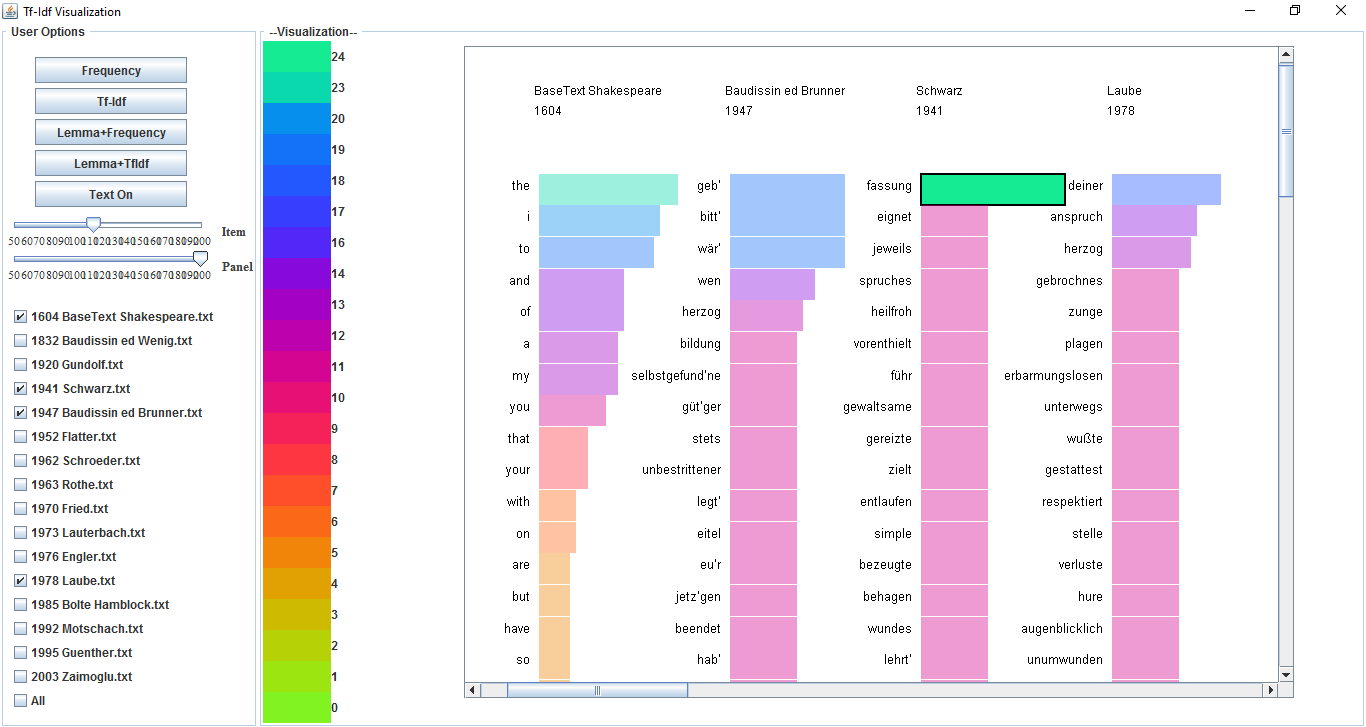
\includegraphics[scale=0.5]{Figs/Fassung}\\[1ex]
	\caption{The word 'fassung' is ranked high Tf-Idf value in one version}
	\label{fig:fassung}
\end{figure} 

\paragraph{Lemmatised View}
\paragraph[]{}Lemmatised View is generated after applying a lemma corpus to process our data. After lemmatisation, words are supposed to change into the original form, namely, the dictionary form (See Implementation chapter for relevant explanation). This feature is designed to combine the same words with different inflected forms. For example, the English word 'you' can be translated into 'dir', 'du', 'sie' and 'euch' in German. Figure \ref{fig:youInFreq} is the result after we select 'you' in the base text concordance. However, in Lemmatised View, only 'ihr' is highlighted.
 
\begin{figure}[H]
	\centering	
	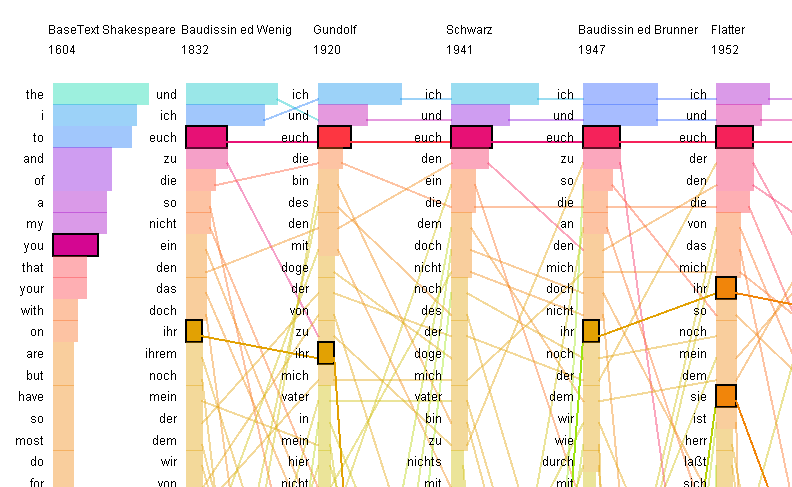
\includegraphics[scale=0.5]{Figs/You-In-Frequency}\\[1ex]
	\caption{ After clicking the block of English 'you' in base text, all German translations in other concordances are highlighted, such as  'dir', 'du', 'sie' , 'euch', and 'euch'.} 
	\label{fig:youInFreq}
\end{figure} 


\begin{figure}[H]
	\centering	
	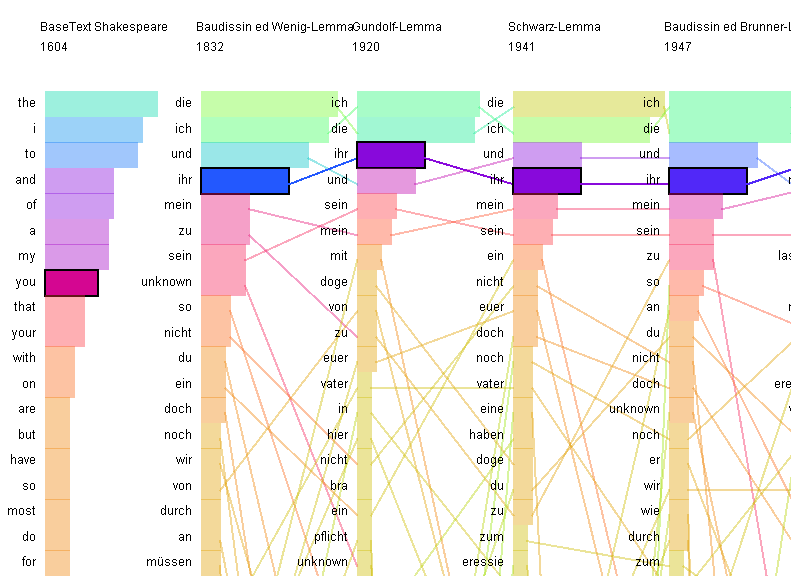
\includegraphics[scale=0.5]{Figs/You-In-Lemma}\\[1ex]
	\caption{After clicking the block of English 'you' in base text, only one German word is highlighted.}
	\label{fig:youInLemma}
\end{figure} 

As a result of lemmatisation, the length of column is shorter in the lemma view than in the frequency view. Also the frequency of words are changed. This can be seen from the colour legend in \ref{fig:freqLemmaComp}. Similarly it can be assumed that the variety of words are more obvious. However, more proofs and interpretations need to be explored in the future.

\begin{figure}[H]
	\centering	
	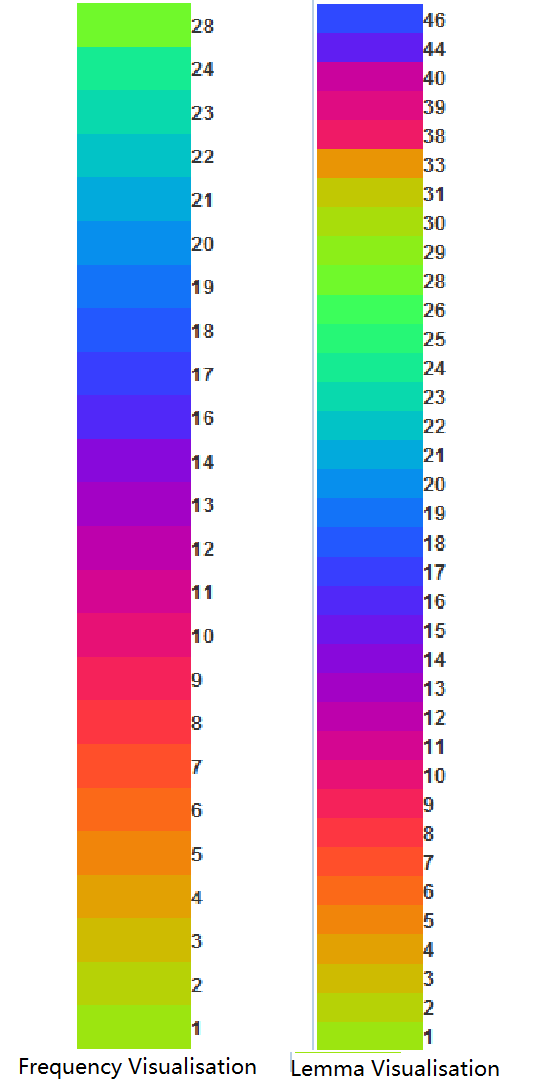
\includegraphics[scale=0.4]{Figs/Freq-Lemma-Comparison}\\[1ex]
	\caption{After combining the inflected form of words, the frequencies are incremented.} 
	\label{fig:freqLemmaComp}
\end{figure} 

\paragraph{Lemmatised Tf-Idf View}
\paragraph[]{} The last view we rendered is the Lemmatised Tf-Idf View. In this view, both the techniques of lemmatisation and Tf-Idf are utilized to display a parallel translation comparison in the software. From this visualisation, not only can we see the dictionary words, but the stop words are filtered. To prove the advantages of these results, two comparisons is necessary:
\begin{itemize} 	
	\item \textbf{Tf-Idf View vs Lemmatised Tf-Idf View}\\
    The German word 'wen', meaning 'whom' in English, which bears little content information but merely performs grammar function. In Tf-Idf visualisation of Figure \ref{fig:tfIdfView}, the word 'wen' ranked on the top of second version from the left which is written by Baudissin ed Wenig in 1832 \cite{Hotho2005}. However, in Figure28, which applied both lemmatisation techiniques and Tf-Idf algorithm, this word disappears. This can be caused by the virtue that the word is combined with the dictionary word of 'wen', which has low Tf-Idf value.
	\item \textbf{Lemmatised View vs Lemmatised Tf-Idf View}\\
If we only apply lemmatisation in the visualisation, stop words are still present. In Figure \ref{fig:lemmaView}, words such as 'die'('the' in English), 'ich'('I' in English), and 'und'('and' in English) are all considered as stop words \cite{Hotho2005}, which contribute little in translation studies. In the Lemma and Tf-Idf view, these words have disappeared because they are ranked to the bottom. 
\end{itemize}

\subsection{Domain Expert Feedback}

A domain expert, Dr. Tom Cheesman from the College of Art and Humanities at Swansea University, was invited as the user to give feedback on this project. During the meetings, we demonstrated the visualisations and features to him. The first one was organised on 13th November, 2017. Following the feedback, some features were overwritten and several new features were developed. The second meeting was on 4th December, 2017, in which he approved the new features.

\subsubsection{Session 1}

At this stage, High Freuency View was finished, along with features such as turning the visualisation on and off, scaling the frame, version selection, and colour legend were implemented. Dr. Tom Cheesman expressed his interest by leaning his body to watch closer to 
the laptop. He asked some questions such as "What do the numbers beside colour legend represent?", "What are the connections?". He also requested that only the base text and three other German translations were shown so that he could understand the alignments. In the feed back, words like 'interesting', 'useful' and 'good' were used a lot. Meanwhile, other suggestions were mentioned and discussed, such as filtering stop words and seeing the most important words, together with showing the lemma of the words to decrease inflected words.

\subsubsection{Session 2}

In this stage, according to the feedback Dr. Cheesman gave at the first meeting, we did some more changes for the project: utilizing Tf-Idf algorithm in data processing, and using the German lemma corpus to lemmatize the terms. 

In the meeting, Dr. Cheesman expressed his interest and excitement by saying "This is good, this is pulling up some interesting stuff", "This is great...I can play with this". He showed great interest in the Lemma and Tf-Idf view, and pointed out some remarkable translations such as abbreviation words in the version written by Baudissin ed Brunner in 1947, (See Figure \ref{fig:feedback}). From the view, we can tell that more abbreviation words are used in this version which implies there is a unique translation strategy which the author uses. At the end of this meeting, Dr. Cheesman asked for a copy of the tools for assisting his translation studies.

\begin{figure}[H]
	\centering	
	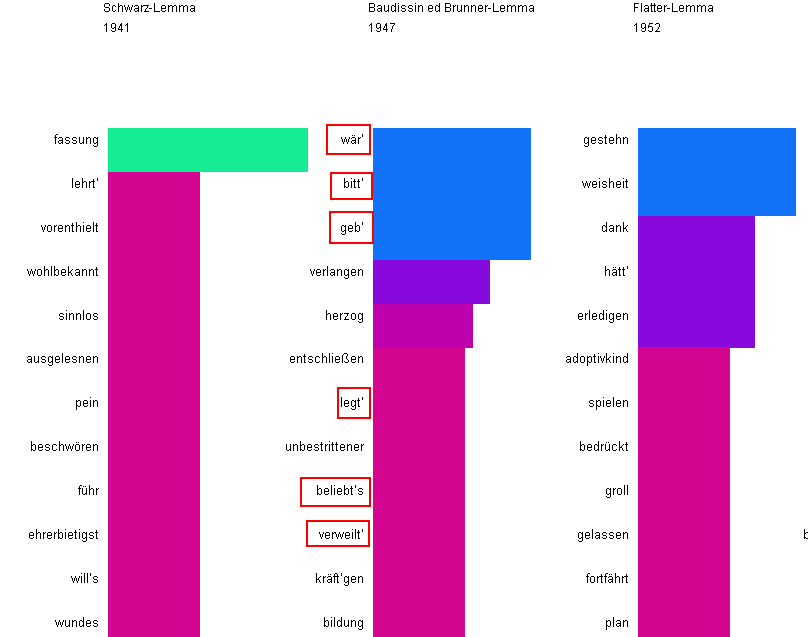
\includegraphics[scale=0.5]{Figs/Marking-Feedback}\\[1ex]
	\caption{After combining the inflected form of words, the frequencies are incremented.} 
	\label{fig:feedback}
\end{figure} 




